\documentclass{article}
\usepackage{tikz}
\usetikzlibrary{arrows.meta,positioning,calc,shapes.geometric}
\pagestyle{empty}
\begin{document}
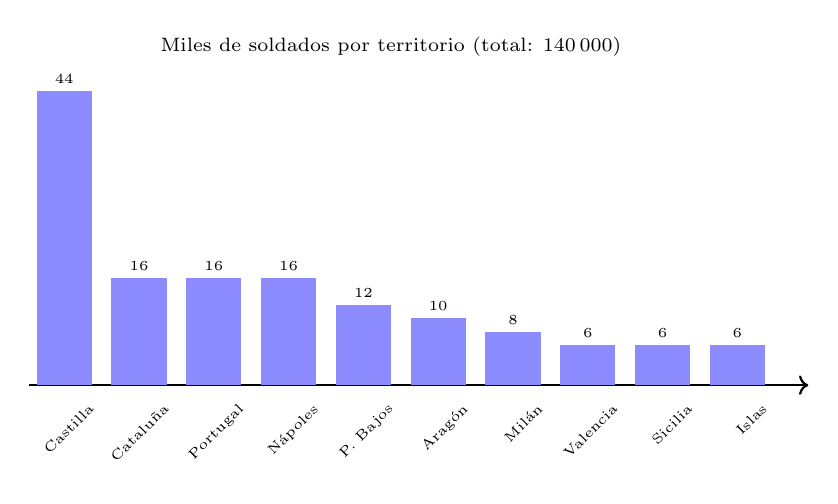
\begin{tikzpicture}
\draw[->, thick] (-0.1,0) -- (9.8,0);
\fill[blue!45] (0.00,0) rectangle (0.70,3.74); \node[font=\tiny] at (0.35,3.89) {44}; \node[font=\tiny, rotate=45, anchor=north east] at (0.65,-0.05) {Castilla};
\fill[blue!45] (0.95,0) rectangle (1.65,1.36); \node[font=\tiny] at (1.30,1.51) {16}; \node[font=\tiny, rotate=45, anchor=north east] at (1.60,-0.05) {Cataluña};
\fill[blue!45] (1.90,0) rectangle (2.60,1.36); \node[font=\tiny] at (2.25,1.51) {16}; \node[font=\tiny, rotate=45, anchor=north east] at (2.55,-0.05) {Portugal};
\fill[blue!45] (2.85,0) rectangle (3.55,1.36); \node[font=\tiny] at (3.20,1.51) {16}; \node[font=\tiny, rotate=45, anchor=north east] at (3.50,-0.05) {Nápoles};
\fill[blue!45] (3.80,0) rectangle (4.50,1.02); \node[font=\tiny] at (4.15,1.17) {12}; \node[font=\tiny, rotate=45, anchor=north east] at (4.45,-0.05) {P. Bajos};
\fill[blue!45] (4.75,0) rectangle (5.45,0.85); \node[font=\tiny] at (5.10,1.00) {10}; \node[font=\tiny, rotate=45, anchor=north east] at (5.40,-0.05) {Aragón};
\fill[blue!45] (5.70,0) rectangle (6.40,0.68); \node[font=\tiny] at (6.05,0.83) {8}; \node[font=\tiny, rotate=45, anchor=north east] at (6.35,-0.05) {Milán};
\fill[blue!45] (6.65,0) rectangle (7.35,0.51); \node[font=\tiny] at (7.00,0.66) {6}; \node[font=\tiny, rotate=45, anchor=north east] at (7.30,-0.05) {Valencia};
\fill[blue!45] (7.60,0) rectangle (8.30,0.51); \node[font=\tiny] at (7.95,0.66) {6}; \node[font=\tiny, rotate=45, anchor=north east] at (8.25,-0.05) {Sicilia};
\fill[blue!45] (8.55,0) rectangle (9.25,0.51); \node[font=\tiny] at (8.90,0.66) {6}; \node[font=\tiny, rotate=45, anchor=north east] at (9.20,-0.05) {Islas};
\node[font=\scriptsize] at (4.5,4.3) {Miles de soldados por territorio (total: 140\,000)};
\end{tikzpicture}
\end{document}
